\begin{enumerate}[label=\thesection.\arabic*.,ref=\thesection.\theenumi]
\numberwithin{equation}{enumi}
\item In a system whose signal flow graph is shown in the figure, $U_1(s)$ and $U_2(s)$ are inputs. The transfer function $\frac{Y(s)}{U_1(s)}$ is

\begin{figure}[!h]
  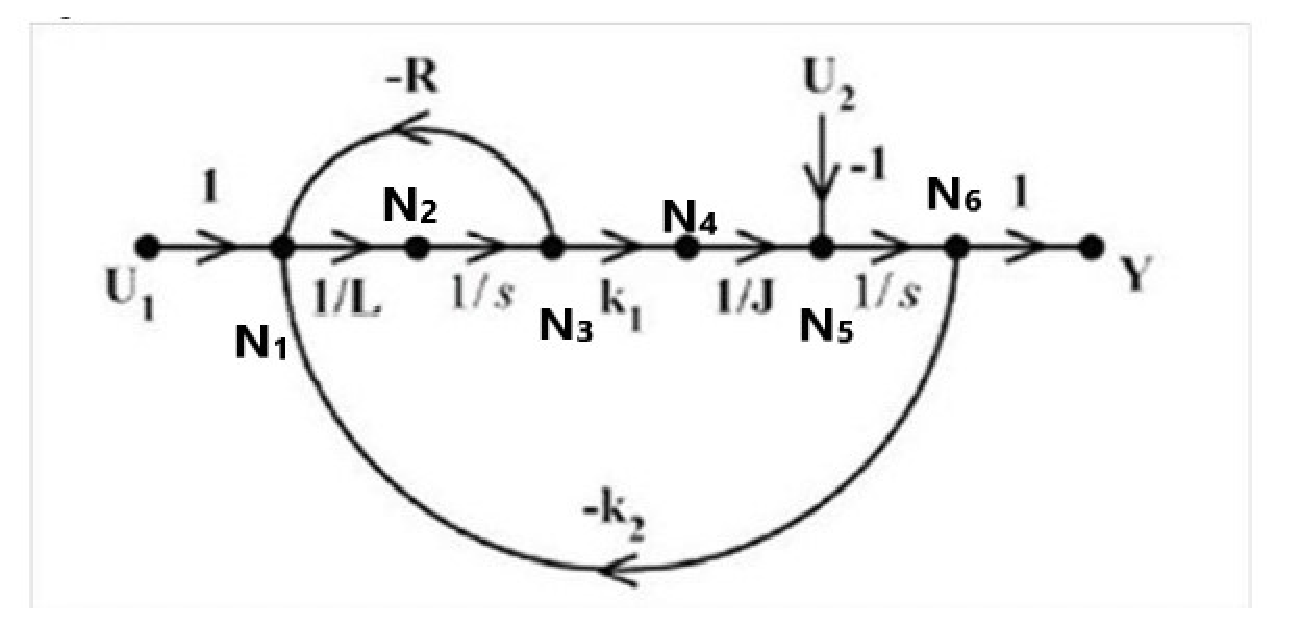
\includegraphics[width=\columnwidth]{picture1.eps}
\end{figure}







\solution 
Using Matrix Formula:
\newline
The transition equations are
\begin{align}
    N1 = U_1-RN_3-k_2N_6  
\end{align}
\begin{align}
    N_2=\frac{N_2}{L}
\end{align}
\begin{align}
    N_3=\frac{N_2}{s}
\end{align}
\begin{align}
    N_4=K_1N_3
\end{align}
\begin{align}
    N_5=\frac{N_4}{J}
\end{align}
\begin{align}
    N_6=\frac{N_5}{s}
\end{align}
State Transition Matrix :
\begin{align}
    \Vec{T} = \myvec{0 & 0 & -R & 0 & 0 & -k_2\\
    \frac{1}{L} & 0 & 0 & 0 & 0 & 0\\
    0 & \frac{1}{s} & 0 & 0 & 0 & 0\\
    0 & 0 & k_1 & 0 & 0 & 0\\
    0 & 0 & 0 & \frac{1}{J} & 0 & 0\\
    0 & 0 & 0 & 0 & \frac{1}{s} & 0}
\end{align}    

\begin{align}
    \Vec{U} = {(1-\Vec{T})^-}^1
\end{align}

\begin{align}
    (1-\Vec{T}) = \myvec{1 & 0 & R & 0 & 0 & k_2\\
    \frac{-1}{L} & 1 & 0 & 0 & 0 & 0\\
    0 & \frac{-1}{s} & 1 & 0 & 0 & 0\\
    0 & 0 & -k_2 & 1 & 0 & 0\\
    0 & 0 & 0 & \frac{-1}{J} & 1 & 0\\
    0 & 0 & 0 & 0& \frac{-1}{s} & 1 } 
\end{align}

${U_5}_0$ will be the gain of the system

\begin{align}
    \Vec{{U_5}_0} = \frac{\mydet{\frac{-1}{L} & 1 & 0 & 0 & 0 \\
    0 & \frac{-1}{s} & 1 & 0 & 0 \\
    0 & 0 & -k_2 & 1 & 0 \\
    0 & 0 & 0 & \frac{-1}{J} & 1 \\
    0 & 0 & 0 & 0& \frac{-1}{s} }}{ \myvec{1 & 0 & R & 0 & 0 & k_2\\
    \frac{-1}{L} & 1 & 0 & 0 & 0 & 0\\
    0 & \frac{-1}{s} & 1 & 0 & 0 & 0\\
    0 & 0 & -k_2 & 1 & 0 & 0\\
    0 & 0 & 0 & \frac{-1}{J} & 1 & 0\\
    0 & 0 & 0 & 0& \frac{-1}{s} & 1 }}
\end{align}

Gain can be found by cofactor expansion or else by running the code in (1.2.5).
Gain obtained is 

\begin{align}
    \frac{Y(s)}{U_1(s)}=\frac{k_1}{s^2LJ+sRJ+K_1k_2}
\end{align}



\end{enumerate}